\documentclass{article}
\usepackage[utf8]{inputenc} % Better fonts
\usepackage{graphicx} % Show images
\usepackage{float} % Allow floats (e.g. Images, Tables)
\usepackage{hyperref} % Links

\usepackage{fancyhdr} % Running header at the top
\usepackage[a4paper, top=3cm, bottom=2.5cm, left=2.2cm, right=2.2cm]%
{geometry}

% Replace "ADD TEAM NUMBER" with your team number
\newcommand{\team}{ADD TEAM NUMBER}

\title{Homework Template}
\author{Automated Learning and Data Analysis \\ 
Team \team \\
TEAM MEMBER 1 NAME, unityID \\
TEAM MEMBER 2 NAME, unityID \\
TEAM MEMBER 3 NAME, unityID \\
}
\date{\today}

\lhead{Team \team}
\chead{Homework ADD NUMBER} % Update the homework number
\rhead{\today}
\pagestyle{fancy}



\begin{document}

\maketitle

\section*{Section Without a Number}

Example of a bulleted list:
\begin{itemize}
    \item Item 1
    \item Item 2
    \item  \textbf{For complex tables:} Use \url{https://www.tablesgenerator.com}
     % This is how you make a comment in LaTeX
\end{itemize}

\section{Section with a Number}

Example of a numbered list:
\begin{enumerate}

\item Example of an nested list

\begin{enumerate}

    \item Classify the following attributes as \emph{nominal, ordinal, interval} or \emph{ratio}. Also classify them as \emph{binary}\footnote{ binary attributes are a special case of discreet attributes},  \emph{discreet} or  \emph{continuous}. If necessary, give a few examples of values that might appear for this attribute to justify your answer. If you make any assumptions in your answer, you must state them explicitly. 
    \begin{enumerate}  
        \item Item 1
        \item Item 2
    \end{enumerate}

    Example of a figure:
    \begin{figure}[H]
    \centering
    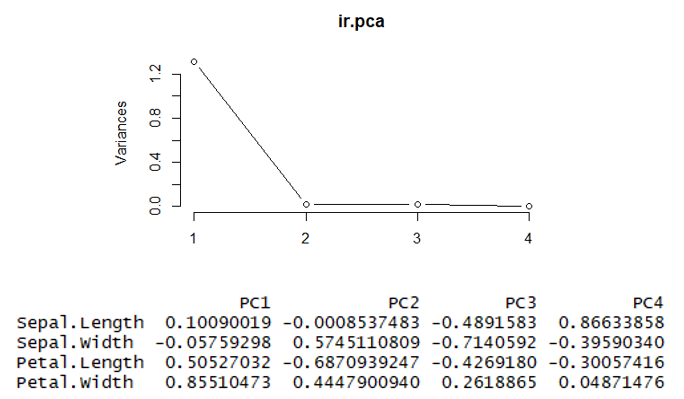
\includegraphics[width=12cm]{PCA1.png}
    \caption{Use \texttt{includegraphics} to add an image}
    \label{PCA1}
    \end{figure}

    \item Example of a Table
    \begin{table}[H]
    \centering
    \caption{Example Table. Note, if you want to make \LaTeX tables, you should probably use \url{https://www.tablesgenerator.com/}}
    \label{automobile}
    \begin{tabular}{llllll}
    \\
     \textbf{Make} & \textbf{Fuel-type} & \textbf{\# of doors} & \textbf{Height}& \textbf{\# of Cylinders}& \textbf{Price} \\
    alfa-romero	& gas	& two &	48.8	&four&	\$1349\\
    alfa-romero&	diesel&	four&	50.52&	six&	\$16500\\
    alfa-romero	&diesel	&two&	54.3&	four&	\$16500\\
    audi&	gas	&four&	55.7&	eight&	\$13950\\
    audi&	diesel&	two	&70.38&	eight&	\$17450\\
    audi&	gas	&four&	71.74&	six&	\$15250\\
    bmw	&diesel	&two&	55.1&	four&	\$16430\\
    bmw&	gas	&four&	54.3&	eight	&\$116925\\
    bmw	&diesel&	two&	53.33&	six	&\$20970\\
    bmw	&diesel&	four&	53.3&	six	&\$21105
    \end{tabular}
    \end{table}

    \item Reference to Table~\ref{automobile}.
  

    \item This is a citation \cite{ganesan2012opinion}.

\end{enumerate}

\end{enumerate}

\bibliographystyle{IEEEtran}
\bibliography{hw1/hw1}
\end{document}
